\chapter{Theoretical Basis}

\section{Background Theory}%
\label{sec:background_theory}
Here we go deeper into the theory of certain elements of the system.

\subsubsection{Bang-Bang CDR}%
\label{ssub:clock_and_data_recovery}
Commonly a serial data stream is sent over a channel without a clock signal.
Clock and Data Recovery (CDR) is the process of extracting timing information
from a serial data stream, then using it to decode the received data stream.  A
CDR circuit has two primary functions. The first is to extract a clock based on
the input data, and the second is to resample the data. 

To extract the clock from the data, a local clock is generated, then is adjusted
as "early" or "late" when compared with the incoming data
signal \cite{sun1989analog}.  We can think of this as a control system, as
shown in Figure~\ref{fig:cdr_basic}.

\begin{figure}[ht]
    \centering
    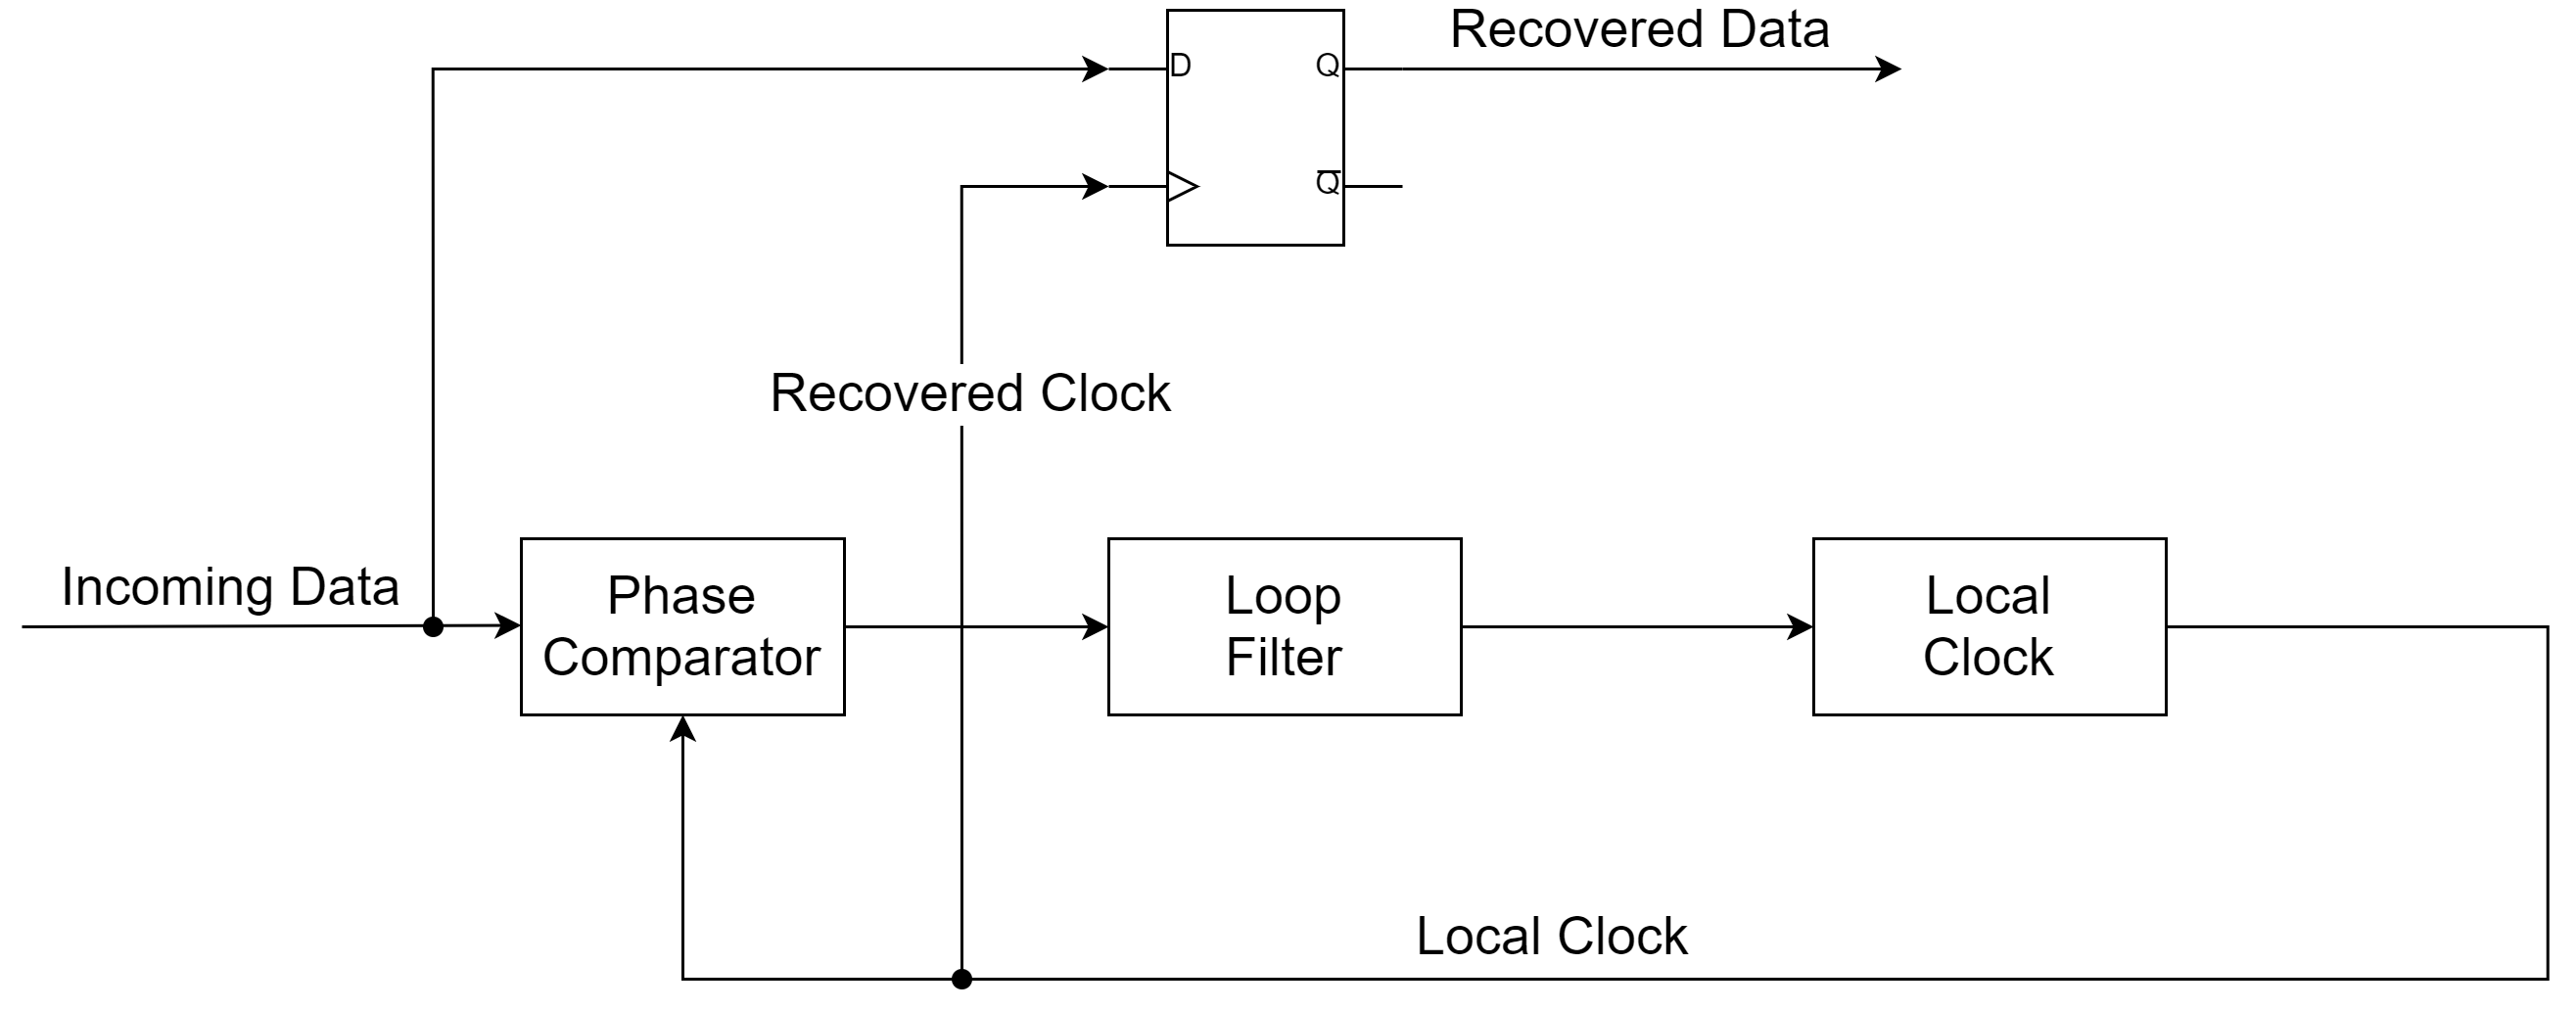
\includegraphics[width=1\linewidth]{img/cdr_basic.png}
    \caption{Basic CDR design}%
    \label{fig:cdr_basic}
\end{figure}

Phase detectors can be divided into two types, linear (where the output has a
linear relationship to the input) and binary or bang-bang phase detectors (where the output
is either positive or negative). Binary phase detectors are more commonly used
in digital CDR circuits~\cite{ZHANG2015163}. An example of one is the
Alexander detector \cite{alexander1975clock} which gives out a high D0+ and a low D0- if the
clock lags and vice-versa if the clock leads, as shown in
Figure~\ref{fig:bang_bang}.

\begin{figure}[ht]
    \centering
    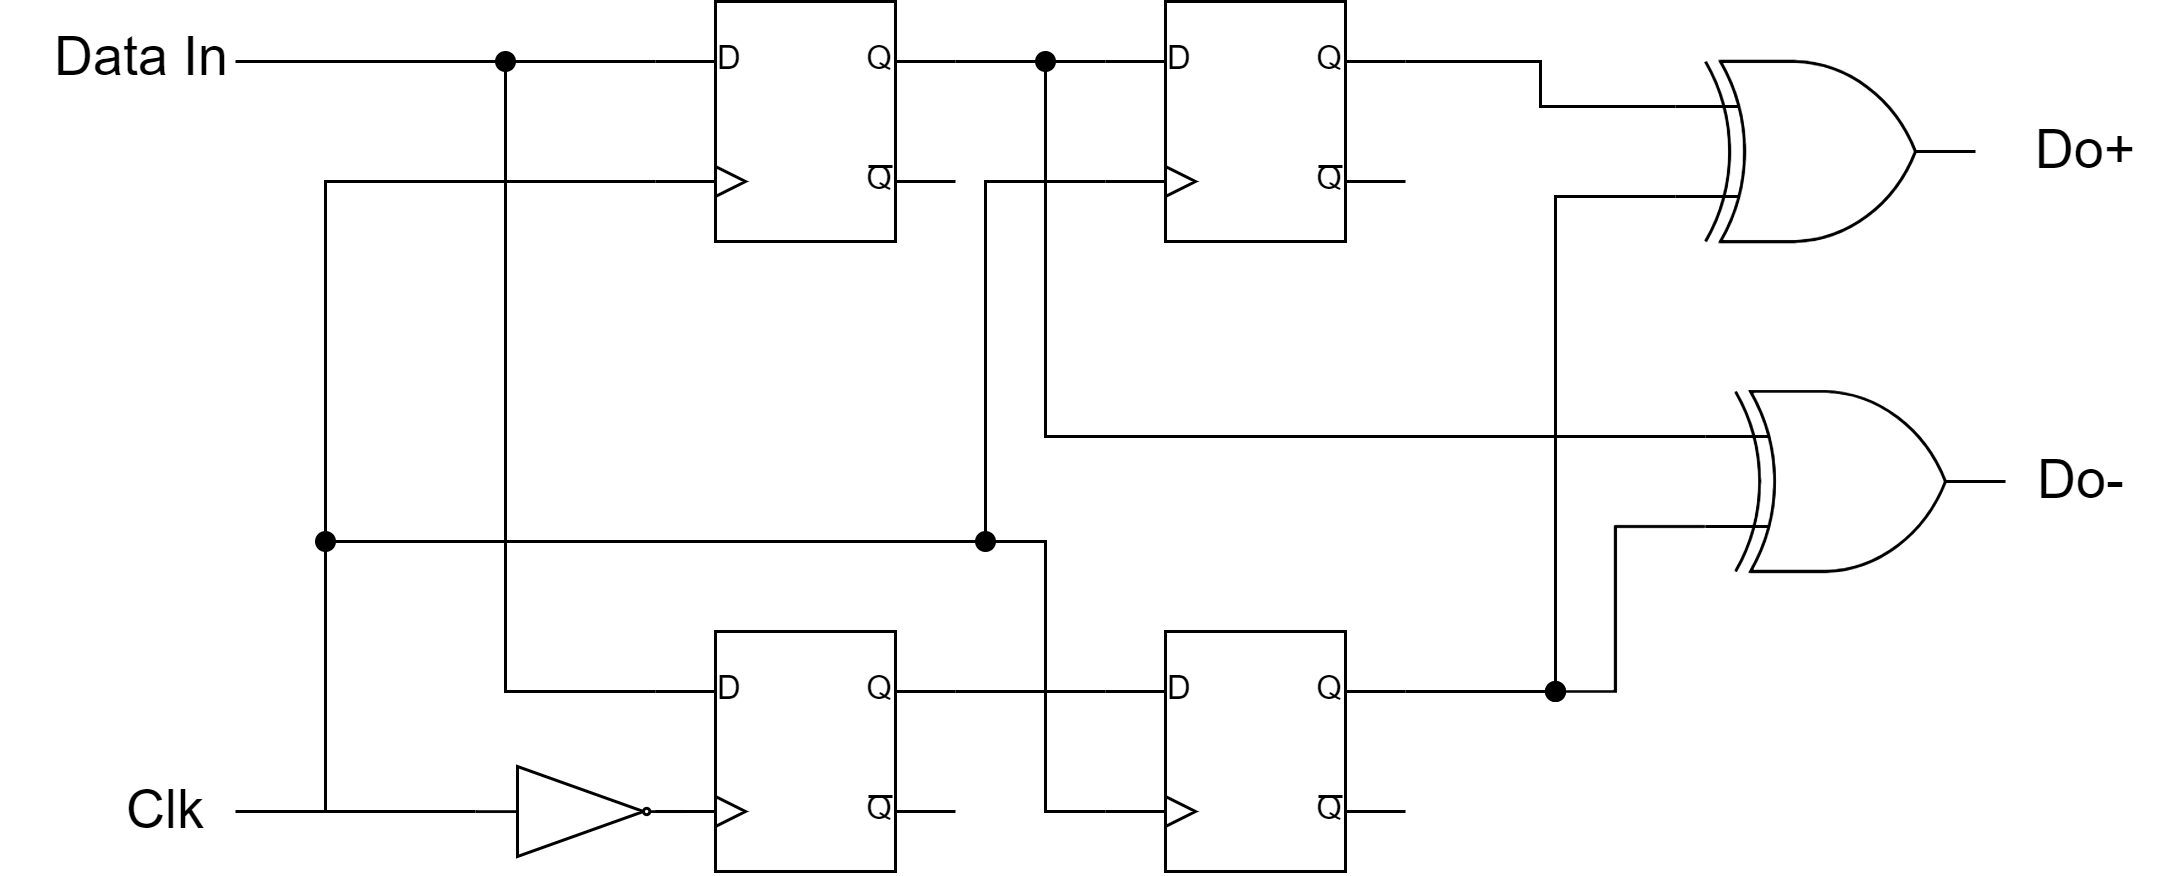
\includegraphics[width=0.8\linewidth]{img/bang_bang.png}
    \caption{Alexander Phase Detector}%
    \label{fig:bang_bang}
\end{figure}

\subsubsection{Pseudorandom Binary Sequence}%
\label{ssub:prbs_generation}
A pseudorandom binary sequence (PRBS) is a sequence of bits that appears to be
random. However as it is generated using a deterministic algorithim, it can be
replicated if the inital conditions are the same.

A common practical implementation of PRBS generation uses linear-feedback shift registers.  As an
example, a PRBS-4 sequence could be generated by using a 4 bit register. We
seed the register with a non-zero number, then tap two bits of the register as
an input. We then shift the contents of the register, taking the last bit as an
output and the new bit as an input, as illustrated in
Figure~\ref{fig:img/shift_reg}.

\begin{figure}[ht]
    \centering
    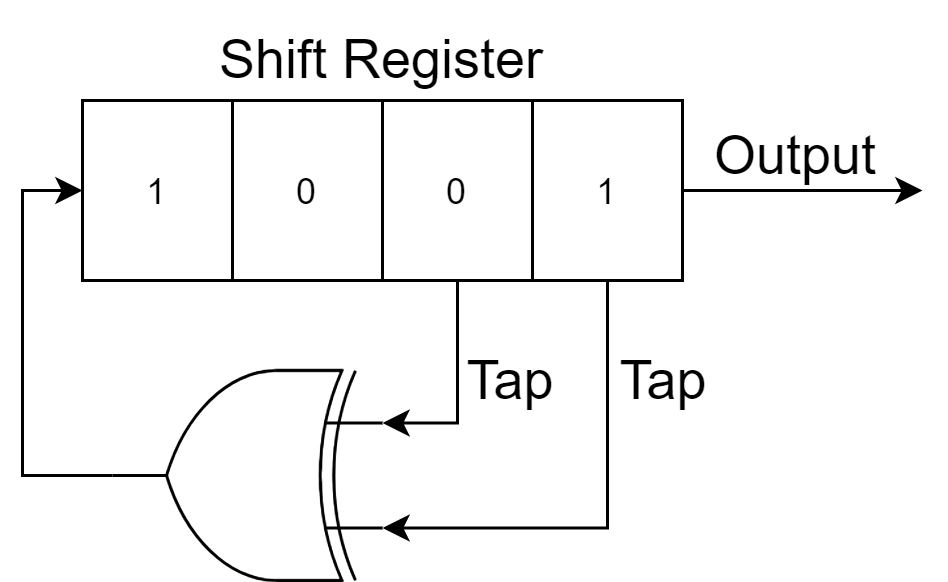
\includegraphics[width=0.4\linewidth]{img/shift_reg.png}
    \caption{Shift Register Implementation}%
    \label{fig:img/shift_reg}
\end{figure}

The full operation can be seen in Table~\ref{tab:shift_reg}. As 0000 cannot
appear (the value of the register would never change) we see that for a register of size N, the
bitsequence is $2^N - 1$ bits long. 
\begin{table}[ht]
    \centering
    \begin{tabular}{|c|c|c c c c|c|}
    \hline
    Cycle & Input & \multicolumn{4}{|c|}{Shift Register} & Output \\
    \hline
     0  & 1 & 1 & 0 & 0 & 1 & 1 \\
     1  & 0 & 1 & 1 & 0 & 0 & 0 \\
     2  & 1 & 0 & 1 & 1 & 0 & 0 \\
     3  & 0 & 1 & 0 & 1 & 1 & 1 \\
     4  & 1 & 0 & 1 & 0 & 1 & 1 \\
     5  & 1 & 1 & 0 & 1 & 0 & 0 \\
     6  & 1 & 1 & 1 & 0 & 1 & 1 \\
     7  & 1 & 1 & 1 & 1 & 0 & 0 \\
     8  & 0 & 1 & 1 & 1 & 1 & 1 \\
     9  & 0 & 0 & 1 & 1 & 1 & 1 \\
     10 & 0 & 0 & 0 & 1 & 1 & 1 \\
     11 & 1 & 0 & 0 & 0 & 1 & 1 \\
     12 & 0 & 1 & 0 & 0 & 0 & 0 \\
     13 & 0 & 0 & 1 & 0 & 0 & 0 \\
     14 &   & 0 & 0 & 1 & 0 & 0 \\
    \hline
    \end{tabular}
    \caption{Shift Register Operation}
    \label{tab:shift_reg}
\end{table}

\subsubsection{Source Synchronous System}%
\label{ssub:source_synchronous_system}
In a source synchronous system a clock signal is provided alongside the data
signal, as shown in Figure~\ref{fig:source_sync}. This has the advantage of not
needing a CDR circuit. Furthermore as both the clock and the data come from the
same device any jitter will be similar across both signals and can likely be
ignored \cite{ragab2011receiver}.   A downside is that there will be crossing
of clock domains at the reciever as the transmitted clock will not be
synchronous with the clock domain of the receiving device.
\begin{figure}[ht]
    \centering
    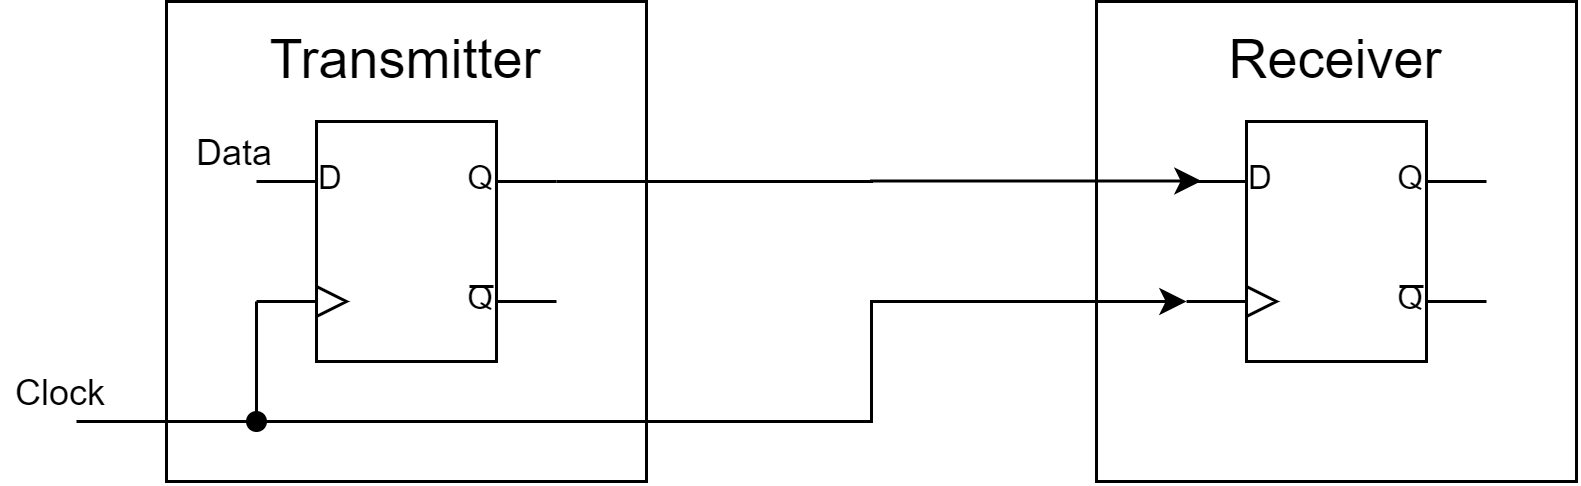
\includegraphics[width=0.5\linewidth]{img/source_sync.png}
    \caption{Source Synchronous System}%
    \label{fig:source_sync}
\end{figure}



\subsubsection{Semiconductor Optical Amplifier}%
\label{ssub:semiconductor_optical_amplifier}
Optical amplifiers are devices that can amplify an optical signal without
needing to convert it to an electrical one. 
A silicon optical amplifier (SOA) is one that uses a semiconductor as the gain
medium, as light passes through this gain medium it is amplified.
SOAs are electrically pumped (do not require the use of another laser) and are of
small size.
\begin{figure}[ht]
    \centering
    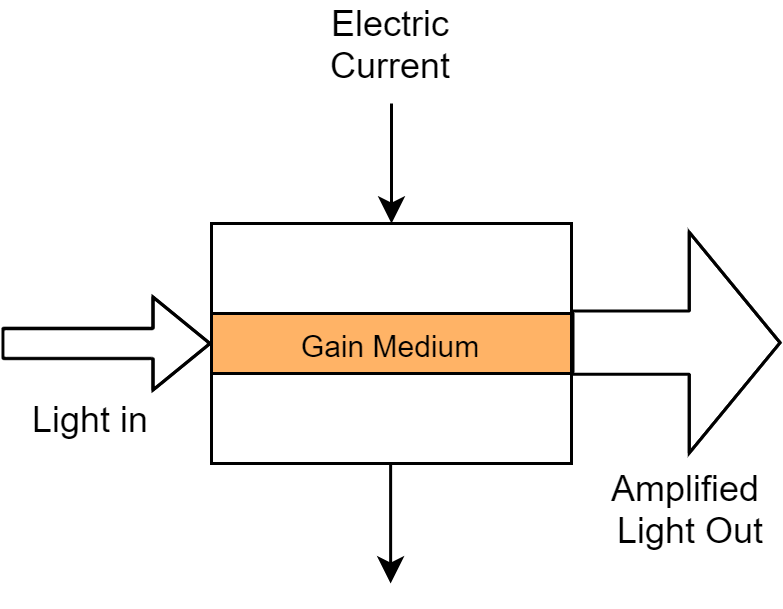
\includegraphics[width=0.4\linewidth]{img/soa.png}
    \caption{Basic SOA Structure}%
    \label{fig:soa}
\end{figure}



\section{Literature Review}%
\label{sec:literature_review}

\noindent \cite{kari_phase} outlines how CDR circuits are a limiting factor in
optical switching and proposes a method of phase caching to overcome this.
The data is transferred over the high-speed Xilinx transceivers, and uses a
bang-bang CDR. The phase measurments that are being compared are that of the
recieved data to the local clock.
The PRBS data is pregenerated (written to memory) and is sent in short bursts
with a known sequence at the end. When the data arrives it is then written to
memory and then processed.  The phase caching improved locking time on
switching by 12 times.

\noindent In \cite{serrano2013white}, \cite{moreira2010digital}, and
\cite{moreira2009white}, the white rabbit project is discussed. A white rabbit
system provides sub-nanosecond synchronisation accuracy. To achieve this,
accurate measurements of the link delay between the nodes of the network must
be calculated.  While instructive, the method is not directly applicable to the
project, as in a White Rabbit system, all the nodes are locked to the same
frequency. Hence the link delay can be calculated by having a node receive a
clock signal from another node, then return the same signal. The link delay can
then be calculated by comparing the phase offset of the two signals.

\noindent \cite{williams2016source} described an optical source synchronous
system. It describes how choosing the correct wavelength for the clock can
minimise the modal cross-talk. Furthermore, in conjunction with
\cite{ragab2011receiver} it describes how source synchronous systems are able
to track correlated jitter between clock and data channels, and how system
performance can be degraded by channel slew between clock and data channels.\\
\cite{williams2019reconfiguration} further explored reducing the modal
crosstalk by proposing an architecture with re-configurable clock and data
paths, thus allowing the user to chose the optimal lane for the sensitive clock
for each photonic interconnect. This may not be needed however, as each
transmitter should have a fixed data characteristic.

\noindent \cite{chen2017optimization} and \cite{fixed_latency} describe fixed
latency links. In the event we were unable to bypass the CDR, it may be
possible to organise the system to have a fixed latency, then force the CDR to
the appropriate fixed phase. Thus the circuit could thus have a much reduced
CDR lock time.

\noindent \cite{dru_guide}, \cite{nidru} describe an Xilinx intellectual
property that allows the high speed serial transceivers to be used at much
lower data rates. This was initially of interest because it would have been
easier to demonstrate a working system with lower data rates. However as this
is an extra IP used in conjunction with the transceivers it did not turn out to
be useful for the project. 

\noindent \cite{mendes_transceiver} this presentation describes a system where
the phase of a transceiver on Xilinx board is kept stable over resets. While
this was done on the transmitter side it shows that fixing the phase of the
transceiver is possible.

